\documentclass[sigconf,anonymous]{acmart}

%% ICAIF '26 submission: double-blind, max 8 pages including figures and references.
%% Camera-ready: remove the `anonymous' option and restore the author block below.

\usepackage{booktabs}

%% --- Project-level numeric macros (carried over from the extended manuscript) ---
\newcommand{\pct}[1]{\ensuremath{#1\%}}
\newcommand{\Kdisc}[1]{\ensuremath{K_{\text{disc}} = #1}}
\newcommand{\LRuc}[1]{\ensuremath{\text{LR}_{\text{uc}} = #1}}
\newcommand{\TIS}[1]{\ensuremath{T_{\text{IS}} = #1}}
\newcommand{\TOoS}[1]{\ensuremath{T_{\text{OoS}} = #1}}
\newcommand{\Prob}{\mathbb{P}}
\newcommand{\E}{\mathbb{E}}
\newcommand{\R}{\mathbb{R}}

\citestyle{acmnumeric}

%% --- Conference metadata ---
\acmConference[ICAIF '26]{7th ACM International Conference on AI in Finance}{November 14--17, 2026}{Milan, Italy}
\acmBooktitle{7th ACM International Conference on AI in Finance (ICAIF '26), November 14--17, 2026, Milan, Italy}
\copyrightyear{2026}
\acmYear{2026}
\setcopyright{acmlicensed}
\acmDOI{10.1145/nnnnnnn.nnnnnnn}
\acmISBN{978-x-xxxx-xxxx-x/YY/MM}

\begin{document}

\title{Heavy-Tail Hidden Markov Generators for Daily Equity Returns: Stylized Facts and Regime-Conditional Value-at-Risk}

%% CAMERA-READY: restore real author block here.
\author{Anonymous Author(s)}
\affiliation{%
  \institution{Anonymous Institution}
  \city{City}
  \country{Country}}
\email{anonymous@example.com}

\renewcommand{\shortauthors}{Anon.}

\begin{abstract}
Synthetic generators of daily US-equity returns support stress testing, regulatory backtesting, and scenario design, none of which a single realized market history can supply on its own. Deep generative models offer capacity at the cost of interpretability, while low-state-count hidden Markov models (HMMs) with Gaussian emissions were long held unable to reproduce the slow autocorrelation decay of absolute returns. We revisit that negative result with a continuous-emission HMM whose latent regime chain governs the autocorrelation while per-regime densities govern the marginal, separating the temporal and distributional channels of the low-state Gaussian limitation. A unified expectation--maximization framework places Gaussian, Student-$t$, Laplace, and generalized-error emissions under shared forward--backward recursions and quantile-based initialization, and a spectral identity bounds the number of geometric decay modes of the absolute-return autocorrelation by the rank of the centred transition matrix. On SPY and a sector-balanced 30-ticker panel the rank bound is not empirically active at the typical ticker once a few states are used: marginal flexibility, not additional decay modes, explains more of the remaining fit gap. With 12 free parameters at three states, the model reproduces the three symmetric Cont stylized facts, narrows the excess-kurtosis gap left by the Gaussian baseline without a tuning hyperparameter, and supports a regime-conditional Value-at-Risk that is not rejected by joint conditional-coverage tests on held-out data or on most walk-forward folds. An i.i.d.\ bootstrap and a maximum-likelihood hidden semi-Markov benchmark match or exceed the model on raw single-window fit, but carry no latent state for a regime-conditional forecast. The scope is daily US equities in stable out-of-sample periods, with periodic refitting recommended when regimes drift.
\end{abstract}

\begin{CCSXML}
<ccs2012>
<concept>
<concept_id>10010147.10010257.10010258.10010262</concept_id>
<concept_desc>Computing methodologies~Latent variable models</concept_desc>
<concept_significance>500</concept_significance>
</concept>
<concept>
<concept_id>10010405.10010455.10010458</concept_id>
<concept_desc>Applied computing~Economics</concept_desc>
<concept_significance>500</concept_significance>
</concept>
<concept>
<concept_id>10002950.10003648.10003688.10003696</concept_id>
<concept_desc>Mathematics of computing~Time series analysis</concept_desc>
<concept_significance>300</concept_significance>
</concept>
</ccs2012>
\end{CCSXML}

\ccsdesc[500]{Computing methodologies~Latent variable models}
\ccsdesc[500]{Applied computing~Economics}
\ccsdesc[300]{Mathematics of computing~Time series analysis}

\keywords{synthetic data generation, hidden Markov models, heavy-tailed distributions, regime switching, Value-at-Risk, stylized facts}

\maketitle

\section{Introduction}
\label{sec:introduction}
Synthetic generators of equity-return time series produce plausible sample paths that match the statistical structure of real markets without replaying the single realized history, supporting stress testing, regulatory backtesting, and scenario design against conditions absent from the observed record~\cite{assefa2020generating}. A useful generator should reproduce the three symmetric stylized facts of daily returns at once: heavy-tailed marginals, negligible linear autocorrelation, and slow decay of the autocorrelation function (ACF) of absolute returns~\cite{mandelbrot1963variation, cont2001empirical}. Generalised autoregressive conditional heteroskedasticity (GARCH) models~\cite{engle1982autoregressive, bollerslev1986generalized} capture volatility clustering but not the multi-regime structure of the marginal; i.i.d.\ generators~\cite{efron1979bootstrap} match the marginal but lose temporal persistence; deep generators~\cite{yoon2019timegan, wiese2020quantgan} reproduce some stylized facts at the cost of interpretability and reproducibility. One negative result has shaped two decades of work on regime-switching models. Ryd\'{e}n et al.~\cite{ryden1998stylized} fitted Gaussian-emission hidden Markov models (HMMs) at low state counts and concluded that the slow decay of the absolute-return ACF was the one stylized fact the model could not generate, ``at least not easily by ML estimation'': a finite-state chain produces only exponential ACF decay, and the joint fit, forced to match the remaining properties of the data, did not land on a slow one. Bulla and Bulla~\cite{bulla2006stylized} attributed the failure to the geometric sojourn-time distribution of the standard Markov chain and recovered the ACF fit with a hidden semi-Markov chain, at the cost of much greater complexity. We separate the low-$K$ Gaussian limitation into two possible failure channels: a temporal one (the absolute growth-rate ACF must allow slow-decay modes) and a distributional one (the marginal mixture must carry enough components to match observed excess kurtosis). Ryd\'{e}n's own outlier-reduced subseries broke on the temporal channel; on our non-outlier-reduced data the distributional channel binds instead. A standard closed-form identity for the absolute growth-rate ACF, written as a sum over the non-unit eigenvalues of the transition matrix~\cite{hamilton1994time, timmermann2000moments}, bounds the number of decay modes by the rank of the centred transition matrix. We ask whether that bound actually matters on equity-return data once enough latent states are allowed.

We answer this with an established model class, the continuous-emission hidden Markov model (CHMM): a hidden chain of market regimes in which each regime emits the day's growth rate from its own probability distribution. The regime chain controls the geometric modes available to the absolute growth-rate ACF, while the per-regime distributions control the heavy-tailed marginal, allowing the temporal and distributional constraints of the low-state Gaussian fit to be examined separately. Our contribution is not the CHMM itself. It is a unified comparison of Gaussian, Student-$t$, Laplace, and generalized-error emissions under the same forward--backward framework; quantile-based initialization, which seeds each regime with its own slice of the observed distribution so the fit converges with every regime still in use; an empirical spectral diagnosis of when the finite-mode bound is active; and a regime-conditional Value-at-Risk (VaR) head that forecasts tail risk from the model's running estimate of which regime the day belongs to. Against deep generative baselines, the fitted model competes at a parameter budget small enough to inspect: 12 free parameters at three states, against the orders-of-magnitude larger convolutional generator--critic architecture of QuantGAN~\cite{wiese2020quantgan}, with each per-state location, scale, and shape directly readable as an economic regime.

We evaluate on a six-fold rolling-origin walk-forward over a decade of SPY and on a sector-balanced 30-ticker panel across ten Global Industry Classification Standard (GICS) sectors, reducing reliance on a single window or asset universe. With enough latent states and a heavy-tailed emission, the model reproduces all three symmetric Cont stylized facts and narrows the excess-kurtosis gap left by the Gaussian baseline. Under the diagnostics used here, the rank bound from the ACF identity is not empirically active at the typical ticker, although a finite-state HMM still permits only finitely many geometric decay modes and the result does not establish a general power-law or multi-scale approximation. The regime-conditional VaR is not rejected by the Christoffersen joint conditional-coverage test~\cite{christoffersen1998evaluating} on the main window or on most walk-forward folds. We therefore interpret the Ryd\'{e}n low-state-count failure more narrowly: on these daily US-equity data and metrics, increasing marginal flexibility resolves more of the observed fit gap than adding ACF modes beyond the selected state count. An i.i.d.\ bootstrap and a maximum-likelihood hidden semi-Markov model (HSMM) beat the CHMM on raw single-window fit, but the fitted CHMM additionally supports the regime-conditional risk forecast exercised here. We make no formal privacy guarantee for its synthetic series. The scope is daily US equities: a non-equity stress test on the GLD exchange-traded fund (ETF) broke down under static fitting, and we recommend periodic refit within that scope.


\section{Related Work}
\label{sec:related}
The discrete-state regime-switching tradition opens with Hamilton~\cite{hamilton1989new}, who introduced Markov-switching to economics. Ryd\'{e}n et al.~\cite{ryden1998stylized} fitted Gaussian-emission HMMs at $K = 2$ or $3$ zero-mean states to subseries of the 1928--1991 S\&P~500 index and concluded that the slow decay of the absolute-return ACF was the one stylized fact the model could not generate by maximum likelihood. Bulla and Bulla~\cite{bulla2006stylized} recovered the fit with hidden semi-Markov models, replacing the geometric sojourn with an explicit-duration family at the cost of a duration-augmented forward--backward, and Nystrup et al.~\cite{nystrup2017long} extended the same line to long-memory volatility. The per-state densities used here draw on the maximum-likelihood Student-$t$ formulations of Peel and McLachlan~\cite{peel2000robust} and Liu and Rubin~\cite{liu1995ml}, with the generalized error distribution (GED) providing a continuous shape parameter that interpolates between Gaussian ($p = 2$) and Laplace ($p = 1$). The present paper contributes a common estimation and evaluation framework across these families rather than a new model class, and tests empirically whether the finite collection of eigenvalue-driven ACF modes is adequate on the studied data rather than claiming general long-memory decay.

Conditional-variance models form a parallel line in which the latent state is the volatility process rather than a discrete regime: Gaussian GARCH~\cite{engle1982autoregressive, bollerslev1986generalized}, heavy-tailed innovations~\cite{bollerslev1987conditionally}, and Markov-switching GARCH (MS-GARCH)~\cite{haas2004new}, with the \texttt{MSGARCH} package of Ardia et al.~\cite{ardia2019msgarch} the reference implementation. These classes can produce heavy-tailed predictive distributions and conditional VaR forecasts; unimodality alone imposes no excess-kurtosis ceiling. The distinction relevant here is narrower: the tested CHMM assigns a separate location, scale, and potentially shape parameter to each finite state, whereas the tested conditional-volatility baselines place most regime dependence in the variance recursion, and the empirical comparison separates those specifications on marginal fit and excess kurtosis without establishing structural impossibility for the broader families.

Deep generative market models offer high-capacity distributional and temporal representations, often with less direct state-level interpretation. GAN-based generators require temporal structure in the architecture or training objective to reproduce volatility clustering~\cite{takahashi2019modeling}; prominent examples include TimeGAN~\cite{yoon2019timegan} and the convolutional Wasserstein GAN QuantGAN~\cite{wiese2020quantgan}. We include one in-house QuantGAN implementation---a materially smaller approximation of the reference architecture, not a faithful reproduction---as the deep-generative row of the main panel, read as a negative control on whether that architecture recovers the stylized facts at our sample size rather than as a representative baseline for the whole family; reports of tail mode collapse in GAN-based financial generators~\cite{takahashi2019modeling} motivate the heavy-tail diagnostic but do not establish that failure for every deep formulation. Synthetic-data evaluation is anchored on the framework of Stenger et al.~\cite{stenger2024thinking} and proper scoring rules~\cite{gneiting2007strictly}; the walk-forward evaluation and periodic-refit recommendation draw on the structural-break and online-updating literature~\cite{cappe2011online}.


\section{Model and Estimation}
\label{sec:model}
For ticker $i$ and trading day $j$, with $P_{i,j}$ the session volume-weighted average price (VWAP), $\Delta t = 1/252$ the annualised trading-day step, and $r_f$ the risk-free rate, the annualised growth rate is
\begin{equation}
    G_{i,j} \equiv \left(\frac{1}{\Delta t}\right) \ln\!\left(\frac{P_{i,j}}{P_{i,j-1}}\right) - r_f.
    \label{eq:growth_rate}
\end{equation}
We set $r_f = 0$ throughout, so $G_{i,j}$ is the annualised log growth rate rather than an empirically risk-free-adjusted excess return. Since $\Delta t$ is fixed, the growth rate is a constant positive multiple of the day's log return; the excess kurtosis and autocorrelations that define the stylized facts are invariant to the rescaling, so the absolute growth-rate ACF measures the same slow-decay stylized fact the literature reports for absolute returns.

The model is fit one ticker at a time; we write $G_t$ for the daily annualised growth rate of the ticker being fit. The sequence $\{G_t\}$ is the observed output of a CHMM with $K$ latent states, $\mathcal{M} = (\mathcal{S}, \mathbf{T}, \mathbf{F}, \boldsymbol{\pi})$~\cite{rabiner1986introduction}: state space $\mathcal{S} = \{1, \ldots, K\}$ with latent state $s_t$, transition matrix $T_{ij} = \Prob(s_{t+1} = j \mid s_t = i)$, initial distribution $\pi_k = \Prob(s_1 = k)$, and per-state emission densities $\mathbf{F} = \{f_k(\,\cdot\,;\boldsymbol\theta_k)\}_{k=1}^K$ with per-state CDFs $F_k$ used in the filter-conditional VaR construction. The risk head is \emph{filter-conditional}: it conditions on the observed return history through the forward filter while integrating over the latent state, so the VaR at level $\alpha$ is the $\alpha$-quantile of the one-step-ahead predictive mixture
\begin{equation}
    p(G_{t+1} \mid G_{1:t}) \;=\; \sum_{k=1}^{K} \Prob(s_{t+1} = k \mid G_{1:t})\, f_k(G_{t+1}; \boldsymbol\theta_k),
    \label{eq:filter_var}
\end{equation}
which moves as the regime belief updates. It is not the state-specific quantity $\operatorname{VaR}_\alpha(G_{t+1} \mid s_{t+1} = k)$, and it is distinct from CVaR/expected shortfall and from the Christoffersen conditional-coverage backtest criterion. With $\bar{\boldsymbol\pi}$ the stationary distribution ($\bar{\boldsymbol{\pi}} = \bar{\boldsymbol{\pi}}\mathbf{T}$, unique when $\mathbf{T}$ is irreducible and aperiodic), the marginal mixture pools the per-state densities by long-run state occupancy,
\begin{equation}
    f(x) = \sum_{k=1}^{K} \bar{\pi}_k\, f_k(x; \boldsymbol\theta_k), \qquad \bar{\boldsymbol{\pi}} = \bar{\boldsymbol{\pi}} \mathbf{T}.
    \label{eq:mixture}
\end{equation}
Unconditional simulation initialises the chain from $\bar{\boldsymbol\pi}$. The variants share the state-space structure and forward--backward recursions but differ in emission family and in the treatment of the initial distribution (Section~\ref{sec:estimation}): CHMM-N uses Gaussian $f_k = \mathcal{N}(\mu_k, \sigma_k^2)$; CHMM-t uses Student-$t$ $f_k = t_{\nu_k}(\mu_k, \sigma_k)$ with $\nu_k \in [\nu_{\min}, \nu_{\max}]$ (an optional exponential penalty on $1/\nu_k$ is used only in the $\lambda = 20$ sensitivity specification); CHMM-L uses Laplace $f_k = \mathrm{Laplace}(\mu_k, b_k)$; CHMM-GED uses the generalized error distribution $f_k = \mathrm{GED}(\mu_k, \alpha_k, p_k)$, which nests the Gaussian ($p_k = 2$) and Laplace ($p_k = 1$) as interior special cases.

\subsection{Estimation by EM}
\label{sec:estimation}

We estimate $(\mathbf{T}, \boldsymbol\theta_{1:K}, \boldsymbol\pi)$ by expectation--maximization (EM). The forward--backward recursions, and likewise the one-step-ahead forward filters of the risk head, evaluate emission log-densities and normalise by logsumexp in log-space for numerical stability, with a prior fallback retained in the filters against fully underflowed rows. Writing $O_t \equiv G_t$, the E-step computes smoothed posteriors $\gamma_t(k) = \Prob(s_t = k \mid O_{1:T})$ and pair posteriors $\xi_t(i,j) = \Prob(s_t = i, s_{t+1} = j \mid O_{1:T})$ by one forward and one backward pass. All four families share the recursions and a quantile-based initialization: observations are sorted, split into $K$ equal-sized chunks, and state $k$'s initial location and scale are seeded from chunk $k$, with $T_{ij}^{(0)} = \pi_k^{(0)} = 1/K$; this reduces overlap among starting components and helps convergence to non-degenerate $K \ge 3$ fits. The Gaussian fitter holds $\boldsymbol\pi$ fixed at uniform (and excludes it from parameter counts), while the Student-$t$, Laplace, and GED fitters update $\pi_k \leftarrow \gamma_1(k)$; on a single long training sequence $\boldsymbol\pi$ is weakly identified either way. The loop runs until the observed-data log-likelihood changes by less than $10^{-4}$ or an iteration cap is reached; each iteration costs $\mathcal{O}(K^2 T)$ for the recursions and transition update plus the per-family emission updates.

The families differ only in the M-step for $\boldsymbol\theta_k$. For CHMM-N, the classical Baum--Welch update~\cite{baum1970maximization} is closed form:
\[
\mu_k \leftarrow \frac{\sum_t \gamma_t(k)\, O_t}{\sum_t \gamma_t(k)},
\qquad
\sigma_k^2 \leftarrow \frac{\sum_t \gamma_t(k)\, (O_t - \mu_k)^2}{\sum_t \gamma_t(k)}.
\] For CHMM-t, we use the expectation conditional maximisation (ECM) construction of Peel and McLachlan~\cite{peel2000robust} and Liu and Rubin~\cite{liu1995ml}, based on the Gaussian scale-mixture representation $G_t \mid s_t = k, u \sim \mathcal{N}(\mu_k, \sigma_k^2/u)$ with $u \sim \Gamma(\nu_k/2, \nu_k/2)$. The E-step adds the latent-precision expectation
\begin{equation}
    u_{t,k} \equiv \E[u \mid O_t, s_t = k] = \frac{\nu_k + 1}{\nu_k + ((O_t - \mu_k)/\sigma_k)^2},
    \label{eq:tprecision}
\end{equation}
and the M-step updates location and scale in closed form given $\nu_k$,
\begin{equation}
    \mu_k \leftarrow \frac{\sum_t \gamma_t(k)\, u_{t,k}\, O_t}{\sum_t \gamma_t(k)\, u_{t,k}},
    \qquad
    \sigma_k^2 \leftarrow \frac{\sum_t \gamma_t(k)\, u_{t,k}\, (O_t - \mu_k)^2}{\sum_t \gamma_t(k)}.
    \label{eq:tupdate}
\end{equation}
The degrees of freedom $\nu_k$ are then updated by a bracketed one-dimensional search on $[\nu_{\min}, \nu_{\max}]$ over the posterior-weighted marginal objective $Q_k(\nu) = \sum_t \gamma_t(k) \log t_\nu(O_t; \mu_k, \sigma_k)$, adapted from the ECME variant of Liu and Rubin~\cite{liu1995ml}. The headline shared-$\nu$ Student-$t$ variant of Table~\ref{tab:model_comparison} instead constrains $\nu_1 = \cdots = \nu_K = \nu$ and updates the single shape by the same bracketed (golden-section) search over $\nu \in [2.1, 50]$ on the aggregate posterior-weighted objective
\[
Q(\nu) = \textstyle\sum_{t}\sum_{k} \gamma_t(k) \log t_\nu(O_t; \mu_k, \sigma_k).
\] Under the counting convention above, the $K^\star = 3$ parameter budgets are $12$ for CHMM-N ($K(K-1)$ transition plus $2K$ emission parameters, $\boldsymbol\pi$ fixed) and $15$ for the shared-$\nu$ CHMM-t ($12$ plus one shared $\nu$ plus $K - 1$ for the updated $\boldsymbol\pi$). In the HMM this update is a hybrid generalised block-coordinate step on a surrogate objective rather than an ECME observed-likelihood maximisation, so monotone observed-data ascent is not guaranteed by the ECM theory for the Student-$t$ and GED fitters; we assess numerical convergence from the observed-data log-likelihood trace and restore the last finite-likelihood iterate. For CHMM-L, both updates are closed form: $\mu_k$ is a $\gamma$-weighted median and $b_k$ the weighted mean absolute deviation. For CHMM-GED, the M-step uses three sequential numerical block updates (bounded searches for location and shape, closed-form scale), an ECM-style block-coordinate procedure diagnosed from its likelihood trace.


\section{Spectral Diagnostic}
\label{sec:spectral}
The route from the transition matrix to slow ACF decay runs through the spectrum of $\mathbf T$. Let $\mathbf v_k$ and $\mathbf w_k$ denote the right and left eigenvectors of $\mathbf T$ at non-unit eigenvalue $\lambda_k$, normalised biorthonormally ($\mathbf w_k^\top \mathbf v_l = \delta_{kl}$), and let $\sigma_{|G|}^2$ denote the stationary variance of $|G_t|$ under the marginal mixture~\eqref{eq:mixture}. The closed-form bilinear identity for the absolute growth-rate ACF of a stationary CHMM, $\E[|G_t|\,|G_{t+\tau}|] = \mathbf m^\top \mathrm{diag}(\bar{\boldsymbol\pi})\,\mathbf T^\tau\,\mathbf m$ for lags $\tau \ge 1$, with $\mathbf m_k = \E[|G_t| \mid s_t = k]$, and its eigendecomposition over the non-unit eigenvalues of $\mathbf T$ are standard in the regime-switching literature~\cite{hamilton1994time, timmermann2000moments}; at $\tau = 0$ the identity does not apply, since the conditional second moment replaces $m_k^2$. Under irreducibility and aperiodicity of $\mathbf T$ (with $\bar{\boldsymbol\pi}$ its unique stationary distribution), finite per-state second moments, and diagonalizability of $\mathbf T$, the spectral decomposition $\mathbf T^\tau = \mathbf 1\bar{\boldsymbol\pi}^\top + \sum_{k=2}^K \lambda_k^\tau\, \mathbf v_k \mathbf w_k^\top$ subtracts the marginal product to give, for $\tau \ge 1$,
\begin{equation}
    \rho_{|G|}(\tau) = \sum_{k=2}^{K} a_k\, \lambda_k^{\tau},
    \qquad
    a_k = \frac{\big(\mathbf m^\top \mathrm{diag}(\bar{\boldsymbol\pi})\, \mathbf v_k\big)\big(\mathbf w_k^\top \mathbf m\big)}{\sigma_{|G|}^2}.
    \label{eq:acf_normalised}
\end{equation}
This is a real-valued sum of geometric modes at the non-unit eigenvalues of $\mathbf T$; complex-conjugate pairs combine into damped oscillatory modes, and a non-diagonalisable $\mathbf T$ yields polynomial-times-geometric Jordan terms instead. Wherever a dominant-mode share is reported below, it is defined as $\max_k |a_k \lambda_k| / \sum_{k \ge 2} |a_k \lambda_k|$ at lag $1$: a share of the total \emph{absolute} modal contribution, which coincides with a share of $\rho_{|G|}(1)$ itself only when all contributions carry the same sign. Our contribution is purely empirical. We apply equation~\eqref{eq:acf_normalised} to recast the Ryd\'{e}n et al.~\cite{ryden1998stylized} low-$K$ failure on the SPY 2014--2024 instance as a rank statement on $\mathbf T - \mathbf 1\bar{\boldsymbol\pi}^\top$. At $K = 2$, the ACF reduces to the mono-exponential $\rho_{|G|}(\tau) = a_2\lambda_2^\tau$ with $\lambda_2 = T_{11} + T_{22} - 1$: its persistence can be tuned through $T_{11} + T_{22}$ but its shape is restricted to one geometric mode. The fitted SPY $K = 2$ chain confirms this empirically: the single non-unit eigenvalue trivially carries $100\%$ of the lag-1 modal contribution, and it is strongly persistent ($\lambda_2 = 0.94$ for Gaussian emissions, $0.95$ for the shared-$\nu$ Student-$t$), so the slow decay is already present at the lower bound. At $K \ge 3$ the matrix admits multiple non-unit eigenvalues and the marginal mixture admits more components. The empirical results test whether those finite-mode and finite-mixture restrictions are active on the studied data; they do not imply that a finite-state HMM reproduces general power-law or multi-scale decay.


\section{Experimental Setup}
\label{sec:setup}
The single-asset analysis uses daily SPY (SPDR S\&P~500 ETF) VWAP prices from January~3, 2014 to January~3, 2024, a ten-year in-sample (IS) window of $\TIS{2{,}516}$ trading days; January~4, 2024 through April~20, 2026 is held out for out-of-sample (OoS) evaluation, giving $\TOoS{572}$ growth rates for the generator diagnostics. The VaR back-tests additionally prepend the boundary growth rate into the first held-out session, so their forecast count is $573$. Prices are split-adjusted but not dividend-adjusted, from commercial daily-price vendors. Cross-ticker generalisation uses a sector-balanced 30-ticker panel spanning ten GICS sectors with three large-cap representatives each, fit one CHMM per ticker.

The CHMM is benchmarked against one representative per model class, all fit on the same IS window: a plain i.i.d.\ empirical bootstrap~\cite{efron1979bootstrap} as the strongest non-parametric baseline; GARCH(1,1) with Gaussian~\cite{bollerslev1986generalized} and Student-$t$~\cite{bollerslev1987conditionally} innovations; MS-GARCH~\cite{haas2004new} as the closest regime-switching comparator, with a Bayesian re-run via the \texttt{MSGARCH} package~\cite{ardia2019msgarch}; a maximum-likelihood HSMM-N as the explicit-duration reference; and an in-house QuantGAN~\cite{wiese2020quantgan} as the deep-generative negative control. For every model we simulate $1{,}000$ independent paths matching the scored window~\cite{stenger2024thinking}, under deterministic seeds.

We score three primary metrics. The two-sample Kolmogorov--Smirnov (KS) pass rate at $\alpha = 0.05$ counts the fraction of simulated paths whose marginal is not rejected against the observed window; because the asymptotic KS null assumes i.i.d.\ observations while both series carry serial dependence, we read this pass rate as a descriptive marginal-fidelity score rather than a calibrated test. Mean simulated excess kurtosis is read against the observed value on the same window. The mean absolute error between observed and simulated ACFs of absolute growth rates over $L = 252$ lags, computed per path and averaged,
\begin{equation}
    \text{ACF-MAE} = \frac{1}{P}\sum_{p=1}^{P}\frac{1}{L}\sum_{\tau=1}^{L} \left| \hat\rho^{\text{obs}}_{|G|}(\tau) - \hat\rho^{\,\text{sim},(p)}_{|G|}(\tau) \right|,
    \label{eq:acf_mae}
\end{equation}
captures volatility clustering, the third Cont stylized fact~\cite{cont2001empirical}. The VaR panel reports the unconditional Kupiec coverage test~\cite{kupiec1995techniques}, the Christoffersen joint conditional-coverage test~\cite{christoffersen1998evaluating} as the primary backtest, and the Engle--Manganelli dynamic-quantile (DQ) test~\cite{engle2004caviar}, against filtered-bootstrap~\cite{barone1999var} and CAViaR~\cite{engle2004caviar} contenders on the same harness. The cross-generator ranking is robust to the distributional-metric choice across KS, Anderson--Darling, Hellinger, and Wasserstein-1 panels; the continuous ranked probability score (CRPS)~\cite{diebold1995comparing} is reported as a tie-break.


\section{Results}
\label{sec:results}
\subsection{Stylized facts, state count, and the spectral diagnostic}
\label{sec:res_stylized}

All three Cont stylized facts hold on both SPY windows (Figure~\ref{fig:stylized_facts}; Table~\ref{tab:model_comparison}, Observed row): the marginal is heavy-tailed (in-sample excess kurtosis $7.68$, out-of-sample $5.29$), linear autocorrelation in the raw growth rate is negligible, and volatility clustering in $|G_t|$ is persistent. A stationary block bootstrap at mean block length $20$ gives broadly overlapping IS and OoS $95\%$ CIs of $[2.17, 12.40]$ and $[0.90, 8.26]$ on the excess-kurtosis point estimates, so kurtosis targets should be read against the joint envelope rather than the points. Sweeping $K \in \{3, 6, 9, 12, 15, 18, 21\}$ for CHMM-N on the IS window, the $K = 3$ versus $K = 6$ comparison could not be separated under four-fold and six-fold rolling-origin cross-validation (mean held-out log-likelihood differences of $0.007$ and $0.027$ nats per observation, flipping sign between fold designs); with only four or six fold differences we treat these comparisons as descriptive. BIC and CAIC selected $K = 3$, and we chose $K^\star = 3$ as a parsimony choice, while $K = 18$ had a substantially lower mean held-out log-likelihood at both cadences. Absolute growth-rate ACF-MAE was nearly flat across the whole sweep, consistent with equation~\eqref{eq:acf_normalised}: a direct effective-rank diagnostic showed a single non-unit eigenvalue carrying $93.6\%$ of the lag-1 $|G|$ ACF at $K = 18$ on SPY, so the $K - 1$ rank bound did not bind at $K \ge 3$ on this instance. Repeating the diagnostic on the 30-ticker cross-section gave a wider distribution, with cross-ticker median dominant-mode share $0.76$ and minimum $0.326$ (NEM); the rank-non-binding claim is supported at the cross-ticker median rather than as a universal property of equity-return data.

\begin{figure}[t]
\centering
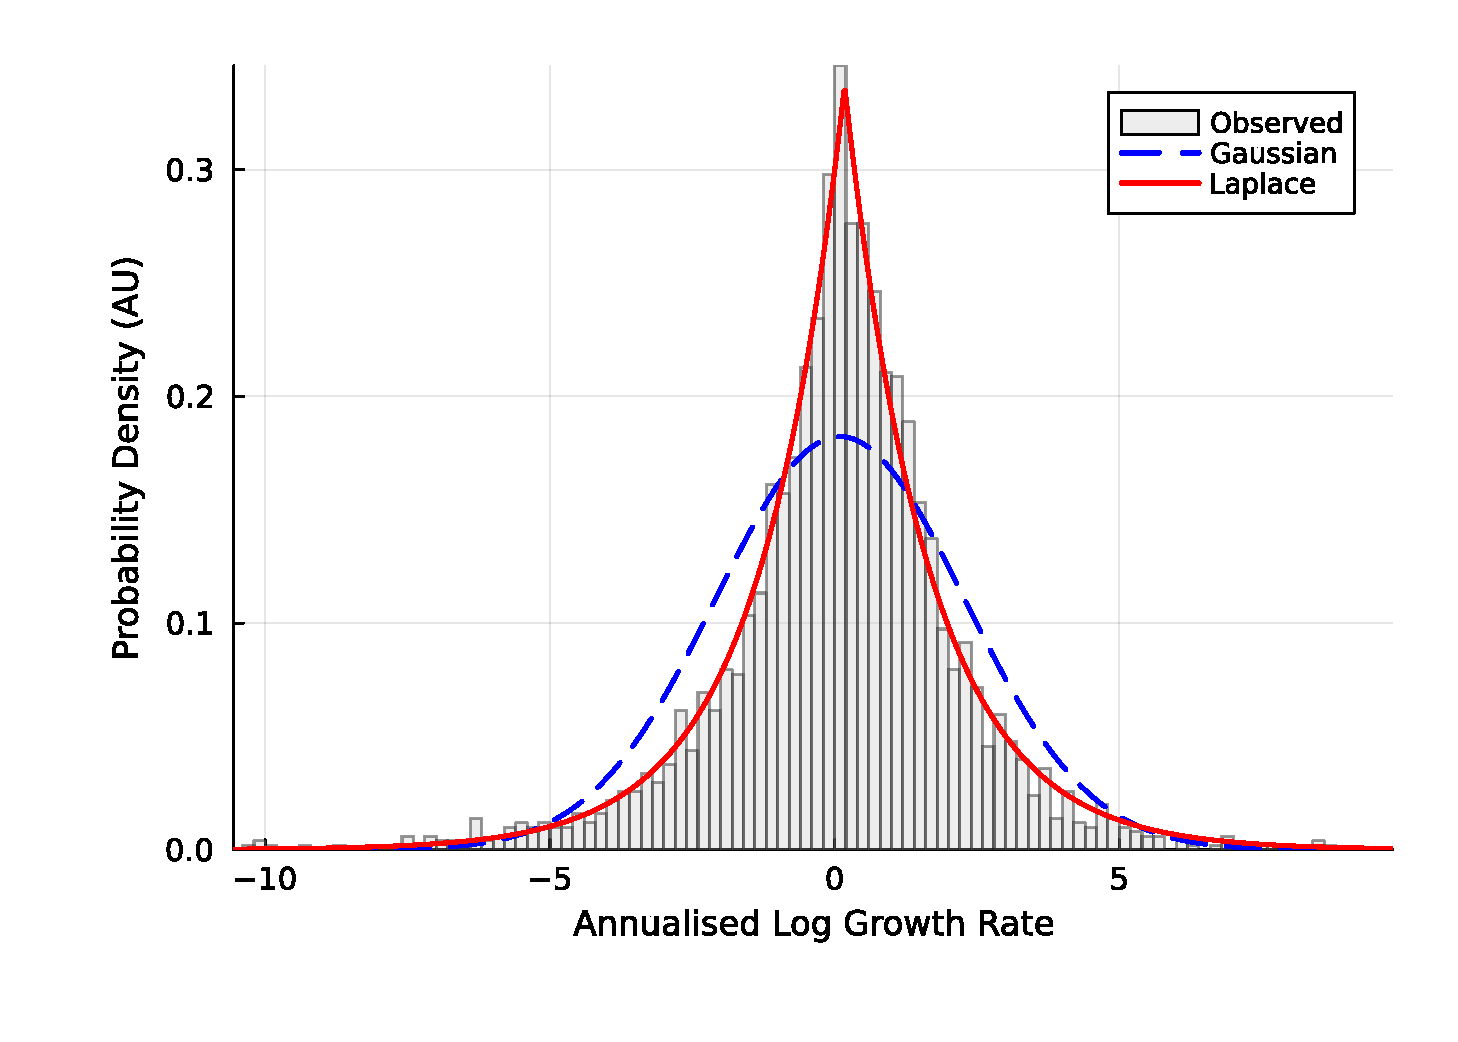
\includegraphics[width=0.49\columnwidth]{figs/Fig-1-Stylized-Facts-a.pdf}\hfill
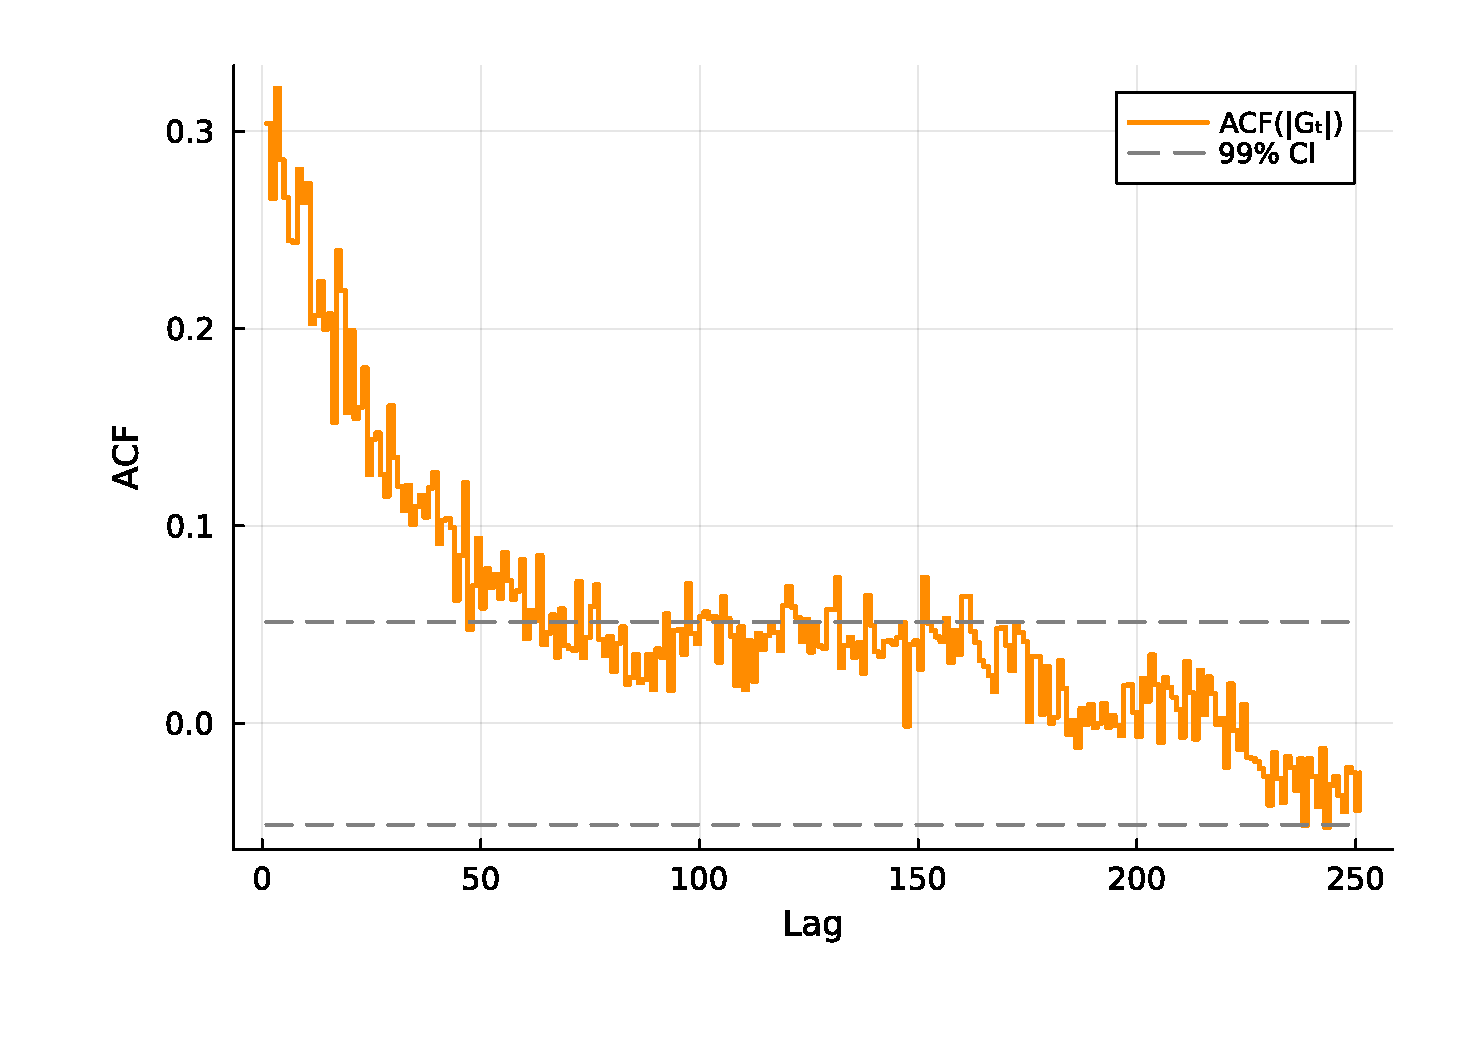
\includegraphics[width=0.49\columnwidth]{figs/Fig-1-Stylized-Facts-d.pdf}
\caption{The two channels of the low-$K$ Gaussian limitation on SPY. Left: heavy-tailed marginal of daily growth rates against Gaussian and Laplace fits (distributional channel). Right: slow decay of the absolute growth-rate ACF (temporal channel).}
\label{fig:stylized_facts}
\end{figure}

\subsection{Generator comparison}
\label{sec:res_generators}

With the state count fixed, we fit the four CHMM variants on the SPY IS window at $K^\star = 3$ and score them against the benchmark generators (Table~\ref{tab:model_comparison}). CHMM-N lands at $91.5\%$ IS and $78.0\%$ OoS KS, simulated excess kurtosis $3.83$ and $3.62$, and $|G_t|$ ACF-MAE $0.0462$ (on par with GARCH at $0.0490$). The shared-$\nu$ Student-$t$ provides the preferred marginal-fit and heavy-tail trade-off, the best CHMM OoS KS together with a smaller kurtosis gap than CHMM-N and no penalty hyperparameter, at $91.9\%$ IS and $82.1\%$ OoS KS with simulated excess kurtosis $4.68$ and $4.46$ against observed $7.68$ and $5.29$; on the kurtosis distance alone the penalty-free CHMM-L and CHMM-GED rows sit closer to observed, at lower KS. (A penalised per-state CHMM-t at $\lambda = 20$, with $\lambda$ tuned at $K = 18$ and re-used at $K^\star = 3$, overshot to IS excess kurtosis $18.87$ through a $1/\nu_k$-shrinkage artefact and is treated as a sensitivity reference only.) The four CHMM variants are statistically indistinguishable on OoS sample-CRPS (from $1.0393$ for CHMM-N to $1.0432$ for CHMM-L, against $1.0398$ for the bootstrap and $1.0440$ for GARCH(1,1)), so the family choice is driven by the per-row kurtosis match. The fitted CHMM matches the slow absolute growth-rate ACF within our lag-252 MAE tolerance on the SPY 2014--2024 instance, where the Ryd\'{e}n et al.~\cite{ryden1998stylized} $K = 2$ to $3$ Gaussian setup judged the ACF fit unsatisfactory, and the raw growth-rate ACF-MAE closes the negligible-linear-autocorrelation fact at $0.0235$ to $0.0240$, indistinguishable from the i.i.d.\ baselines. MS-GARCH stays well below the CHMM on KS under both point-estimate and Bayesian posterior-predictive variants, and the QuantGAN negative control fails all three stylized facts at this sample size ($0.0\%$ KS, excess kurtosis $0.56$, ACF-MAE at the i.i.d.\ floor).

\begin{table}[t]
\centering
\caption{Main generator comparison on SPY: $1{,}000$ simulated paths; IS $T = 2{,}516$, OoS $T = 572$. KS = Kolmogorov--Smirnov pass rate at $\alpha = 0.05$; Kurt = mean simulated excess kurtosis (observed $7.68$ IS, $5.29$ OoS); ACF-MAE over $252$ lags for absolute ($|G_t|$) and raw ($G_t$) growth rates. QuantGAN is the deep-generative negative control; the shared-$\nu$ CHMM-t fits a single $\nu$ across states with no penalty.}
\label{tab:model_comparison}
\footnotesize
\setlength{\tabcolsep}{3.4pt}
\renewcommand{\arraystretch}{0.97}
\begin{tabular}{l cc cc cc}
\toprule
& \multicolumn{2}{c}{KS (\%) $\uparrow$} & \multicolumn{2}{c}{Exc.\ Kurt} & \multicolumn{2}{c}{ACF-MAE $\downarrow$} \\
\cmidrule(lr){2-3} \cmidrule(lr){4-5} \cmidrule(lr){6-7}
Model & IS & OoS & IS & OoS & $|G_t|$ & $G_t$ \\
\midrule
\textit{Observed}     & --     & --     & $7.68$  & $5.29$  & --       & --       \\
Bootstrap             & $99.8$ & $91.8$ & $7.55$  & $6.86$  & $0.0628$ & $0.0235$ \\
GARCH(1,1)            & $27.4$ & $59.6$ & $7.59$  & $2.70$  & $0.0490$ & $0.0244$ \\
GARCH(1,1)-$t$        & $57.3$ & $80.8$ & $15.13$ & --      & $0.0316$ & $0.0173$ \\
MS-GARCH ($K=3$)      & $36.1$ & $33.1$ & $4.10$  & --      & $0.0284$ & $0.0173$ \\
QuantGAN TCN          & $0.0$  & $0.0$  & $0.56$  & $0.53$  & $0.0617$ & $0.0264$ \\
\midrule
CHMM-N                & $91.5$ & $78.0$ & $3.83$  & $3.62$  & $0.0462$ & $0.0240$ \\
CHMM-L                & $80.5$ & $63.6$ & $5.24$  & $5.20$  & $0.0530$ & $0.0235$ \\
CHMM-GED              & $90.3$ & $78.4$ & $5.45$  & $5.09$  & $0.0531$ & $0.0236$ \\
CHMM-t shared-$\nu$   & $91.9$ & $82.1$ & $4.68$  & $4.46$  & $0.0531$ & $0.0236$ \\
\midrule
ML HSMM-N             & $98.4$ & $91.0$ & $3.46$  & $3.38$  & $0.0629$ & $0.0236$ \\
\bottomrule
\end{tabular}
\end{table}

Two benchmark rows beat the CHMM on raw single-window OoS KS: the i.i.d.\ bootstrap ($91.8\%$) and the maximum-likelihood HSMM-N ($91.0\%$). That advantage is confined to the marginal axis: on volatility clustering both rows sit at the i.i.d.\ $|G_t|$ ACF-MAE floor ($0.0628$ and $0.0629$), while CHMM-N clusters below the floor at $0.0462$. The CHMM is the one generator in the panel equipped here with the regime-conditional VaR head: the i.i.d.\ bootstrap is structurally unable to produce a regime-conditional VaR (it carries no latent state), and HSMM-based risk heads are left as a companion-paper direction. A six-fold rolling-origin walk-forward reaches median OoS KS $62.1\%$ at $K^\star = 3$, with two stress folds (W2 COVID, W4 2022 rate-hike onset) below $10\%$ at both tested state counts ($K \in \{3, 18\}$, CHMM-N); we treat the walk-forward median, not the single-window OoS pair, as the right summary for judging live use.

\subsection{Tail index}
\label{sec:res_tail}

Because excess kurtosis is a fragile fourth-moment functional under heavy tails, we complement it with a threshold-local Hill estimate~\cite{hill1975tail} applied identically to the observed series and every simulated family at $K^\star = 3$ (top $5\%$ of $|G_t|$ exceedances); for the light-tailed mixture families this quantity is a shape diagnostic of the estimated threshold range, not an asymptotic tail index. The observed tail index is $\hat\alpha = 3.15$ IS and $3.30$ OoS, inside the $(2, 5)$ band reported by Cont~\cite{cont2001empirical} for daily equity returns, with a block-bootstrap $95\%$ CI of $[2.45, 4.25]$ on the IS estimate. The shared-$\nu$ CHMM-t lands at $\hat\alpha = 3.67$ on both windows with an across-path $95\%$ band of $[3.11, 4.38]$ overlapping the observed CI, so the simulated tail is matched, sitting slightly thinner in the far tail, rather than undershot. Every emission family produces an in-band estimate at $K^\star = 3$ (CHMM-N $3.41$, CHMM-L $3.26$, CHMM-GED $3.24$) even though simulated excess kurtosis spans $3.83$ to $18.87$ across the same rows: at the depths the estimator sees, the regime mixture rather than the emission family carries the heavy tail, while the emission shape governs how far into the extreme tail the match extends. Applied per tail side, the same estimator reproduces the direction of the observed gain/loss asymmetry (observed loss-minus-gain gap $-0.55$; shared-$\nu$ $-0.46$, CHMM-L $-0.44$) from the regime means alone.

\subsection{Cross-ticker generalisation and refit}
\label{sec:res_crossticker}

Fitting one model per ticker on the sector-balanced 30-ticker panel, the in-sample KS distribution is concentrated (median $96.8\%$) and the out-of-sample distribution is wider, with median $69.1\%$, mean $66.2 \pm 28.2\%$, and $11/30$ tickers below $60\%$. The deepest failures are tickers that introduced a new regime out of sample: LLY and UNH in Health Care, NEM in Materials. An ANOVA on OoS KS by sector returned no significant sector effect on either the original $n = 3$ design or an $n = 6$ expansion to a 60-ticker panel, so the visible concentration of failures on regime-introducing tickers is a per-ticker observation rather than evidence of sector-level structure. Periodic refit closes much of the gap: at $K^\star = 3$ a quarterly refit shifts the OoS KS median from $69.1\%$ to $84.7\%$ and reduces failures from $11/30$ to $8/30$. In companion multi-asset experiments, per-asset CHMM marginals compose through a rank-based Student-$t$ copula that reproduces contemporaneous cross-asset correlations (in-sample off-diagonal MAE $0.027$ on a six-asset basket); that construction is cross-sectional only, preserving each asset's marginal and the contemporaneous dependence but not per-asset serial dependence, and is not evaluated further here.

\subsection{Regime-conditional Value-at-Risk}
\label{sec:res_var}

We back-test a regime-conditional VaR built from the CHMM one-step-ahead state forecast: the forward filter runs under IS-fixed parameters $(\mathbf T, \{\boldsymbol\theta_k\})$, only the one-step-ahead state-probability vector updates through the OoS window, and the VaR is the $\alpha$-quantile of the state-mixture predictive. The back-test covers all $573$ held-out forecasts (Table~\ref{tab:cond_var}). At VaR level $\alpha = 0.05$ the CHMM rows are not rejected by Christoffersen-cc ($p_{\text{cc}} \in [0.39, 0.67]$ across CHMM configurations), and CHMM-N at $K^\star = 3$ is likewise not rejected by the DQ test ($p = 0.09$); non-rejection at these sample sizes indicates compatibility with correct conditional coverage rather than a demonstration of it. Breach rates at $\alpha = 0.05$ sit close to nominal, from $26$ breaches ($4.54\%$) at $K = 18$ to $36$ ($6.28\%$) at $K^\star = 3$, and no CHMM row is rejected by Kupiec or Christoffersen-ind at that level. The $\alpha = 0.01$ rows are also not rejected by Christoffersen-cc ($p_{\text{cc}} \in [0.10, 0.16]$) but are power-bounded at $\TOoS{573}$, where only about $5.7$ breaches are expected; the higher-power DQ test separates the state counts, rejecting CHMM-N at $K = 18$ ($p = 0.02$) while $K^\star = 3$ escapes rejection only marginally ($p = 0.06$). Against the two non-state-space contenders the CHMM rows reach approximate parity at $\alpha = 0.05$; at $\alpha = 0.01$ only CHMM-N at $K^\star = 3$ is not rejected by DQ, a power-bounded non-rejection rather than evidence of a significant difference, since failure to reject does not establish the null and no pairwise model-comparison test was conducted. The filtered bootstrap ($p = 0.04$) and CAViaR ($p = 0.01$) are both rejected at that tier, as is every other CHMM family and state count in the full sixteen-row family panel of the extended experiments ($p$ from $0.0005$ to $0.030$). Extending to six rolling-origin walk-forward folds, Christoffersen-cc does not reject on $19$ of $24$ rows at the $5\%$ test level, with the five rejections concentrated on stress folds: all four W2 (COVID 2020) rows reject, while W4 (2022 rate-hike onset) produces a single tail-tier rejection at $K = 18$, $\alpha = 0.01$; we read these multi-row panels as multiplicity-aware descriptive evidence rather than repeated confirmations.

\begin{table}[t]
\centering
\caption{Regime-conditional VaR back-test on SPY OoS ($\TOoS{573}$ forecasts including the boundary return; seed fixed). CHMM rows use the forward filter under IS-fixed parameters; contenders are scored on the same Christoffersen/DQ harness. $\alpha = 0.01$ rows are power-bounded at this sample size; DQ $p$-values use the 4-lag specification.}
\label{tab:cond_var}
\footnotesize
\setlength{\tabcolsep}{5pt}
\begin{tabular}{l c c c c c c}
\toprule
Model & $K$ & $\alpha$ & Breaches & Rate & $p_{\text{cc}}$ & $p_{\text{DQ}}$ \\
\midrule
CHMM-N             & $3$  & $0.01$ & $9$  & $1.57\%$ & $0.14$ & $0.06$ \\
CHMM-N             & $3$  & $0.05$ & $36$ & $6.28\%$ & $0.39$ & $0.09$ \\
CHMM-N             & $18$ & $0.01$ & $9$  & $1.57\%$ & $0.14$ & $0.02$ \\
CHMM-N             & $18$ & $0.05$ & $26$ & $4.54\%$ & $0.67$ & $0.68$ \\
\midrule
Filtered bootstrap & --   & $0.01$ & $8$  & $1.40\%$ & $0.16$ & $0.04$ \\
Filtered bootstrap & --   & $0.05$ & $24$ & $4.19\%$ & $0.43$ & $0.55$ \\
CAViaR (SAV)       & --   & $0.01$ & $6$  & $1.05\%$ & $0.14$ & $0.01$ \\
CAViaR (SAV)       & --   & $0.05$ & $25$ & $4.36\%$ & $0.55$ & $0.76$ \\
\bottomrule
\end{tabular}
\end{table}


\section{Limitations and Conclusion}
\label{sec:conclusion}
The CHMM family, fitted with common forward--backward recursions, family-specific M-steps, and quantile-based initialization, captures the three symmetric stylized-fact diagnostics on daily US-equity returns at $K^\star = 3$, while leaving an excess-kurtosis gap whose size is set by the choice of heavy-tailed emission family. A $K = 2$ replication on SPY localises the binding channel: the IS KS pass rate falls to $79.0\%$ (against $91.5\%$ for CHMM-N at $K^\star = 3$) while the absolute growth-rate ACF-MAE stays essentially constant ($0.0501$ versus $0.0462$) and the fitted $K = 2$ spectrum carries the entire absolute growth-rate ACF in a single persistent mode ($\lambda_2 = 0.942$). On these data, then, the marginal distribution, not the ACF, limits the low-$K$ Gaussian fit. The mechanism is empirical rather than structural: a three-component Gaussian scale mixture can in principle reach arbitrarily high kurtosis through a small-weight, large-variance component, but the joint ML fit, disciplined by the bulk of the data, does not select such a configuration; what a finite Gaussian mixture structurally cannot supply is a genuinely power-law tail, since it remains asymptotically light-tailed at every parameter setting. This reading does not contradict Ryd\'{e}n et al.~\cite{ryden1998stylized}, whose subseries were winsorised at four sample standard deviations, bringing the kurtosis within reach of a Gaussian mixture; on our raw data the marginal channel binds instead. On the ACF we agree with their in-principle limit: a finite-state HMM produces only finitely many geometric decay modes, we match the absolute growth-rate ACF only within our lag-252 MAE tolerance, and the structural fix for genuinely slow decay is the semi-Markov chain of Bulla and Bulla~\cite{bulla2006stylized}.

The scope limits are explicit. A CHMM fit once in sample does not generalise across regime introductions: the GLD non-equity stress and the W2 (COVID) and W4 (2022 rate-hike) walk-forward folds broke down under static fitting, and no tested refit cadence closed those folds, while quarterly refit did recover the non-stress cross-ticker panel (Table~\ref{tab:validation}). We evaluated only the three symmetric stylized facts; the dynamic leverage effect is not modelled, although the regime means recover part of the static gain/loss asymmetry. The i.i.d.\ bootstrap and the moment-updated-duration HSMM-N beat the CHMM on raw single-window OoS KS, a marginal-axis result only, and no formal privacy guarantee is claimed for the synthetic output.

What the small model buys is inspectability. CHMM-N at $K^\star = 3$ has $K(K-1) + 2K = 12$ free parameters and the shared-$\nu$ CHMM-t has $15$, against the orders-of-magnitude larger QuantGAN generator--critic architecture~\cite{wiese2020quantgan}. The fitted states read directly as return/volatility regimes: on SPY the three Gaussian states land at a calm regime ($\mu = 0.29$, $\sigma = 0.85$ in annualised growth-rate units), an intermediate regime ($0.14$, $1.91$), and a stress regime ($-0.43$, $3.98$), with the shared-$\nu$ Student-$t$ adding one global tail-shape parameter ($\nu = 5.81$) rather than a per-state shape; no external economic-state validation is performed. BIC/CAIC and rolling-origin validation select the state count, while the closed-form eigenvalue argument explains why additional decay modes are unnecessary on this instance. Future work includes asymmetric emission families targeting the leverage effect, explicit-duration sojourn laws that escape finite geometric memory, online change-point detection against the stress folds, and multi-asset composition through a serial-dependence-preserving copula layer. Code, fitted models, and the runner scripts that regenerate every reported table will be released publicly upon publication; daily prices are from commercial vendors and are not redistributed.


\bibliographystyle{ACM-Reference-Format}
\bibliography{references}

\end{document}
